\documentclass[10pt,letterpaper]{ltugboat}
\usepackage{times,amsmath,graphicx,array,listings,ragged2e}
\usepackage[german,english]{babel}
\usepackage{verbatim}
%
\title{Using \MP { }to create a basic sewing pattern from individual measurements}
%
\author{%
{Dolores Messer{\small $~^{1}$}, Marium Zeeshan{\small $~^{2}$}, Prasenjit Saha{\small $~^{3}$}}%
% add some space between author names and affils
\vspace{1.6mm}\\
\fontsize{10}{10}\selectfont\itshape
$^{1}$\,$^{2}$\,$^{3}$\,Institute for Theoretical Physics, University of Zurich, Switzerland\\
\fontsize{9}{9}\selectfont\ttfamily\upshape
\\
$^{1}$\,dolores.messer@uzh.ch\\
$^{2}$\,marium.zeeshan@uzh.ch\\
$^{3}$\,psaha@physik.uzh.ch
% add some space between email and affil
\vspace{1.2mm}\\
\fontsize{10}{10}\selectfont\rmfamily\itshape
}
%%%%%%%

\begin{document}
\maketitle
%%%%%%%
\lstset{language=MetaPost}
%%%%%%%
\begin{abstract} 
\textit{Generate bodice sloper with \MP. General outcome: Can be done without problems if body shape is not special. Very sensitive to measurement errors. Challenge: dart creation, smooth transitions.}
\end{abstract}
%%%%%%%

%%%%%%%
\section{Introduction}
\par Sewing is one of the oldest textile arts, which is passed from generation to generation. For thousand of years, sewing has been done by hand using needles, whereas nowadays almost all sewing is done by sewing machines. Before a piece of clothing can be sewn together, the parts of the garment are traced onto fabric using a pattern and then cut out. The construction of the pattern is one of the more difficult tasks of the sewing process. Simple patterns are just based on specific measurements of the intended wearer, whereas more complex patterns involve a special design. There are basic patterns, called slopers, which are made to fit a particular individual exactly. From this basic pattern, other patterns can be drafted by pattern manipulation techniques. As the exact measurements vary from person to person, a sloper is different for each person. Since the basic construction of a sloper is done the same way for each individual, a lot of cumbersome work could be avoided by automating this process. Ideally, some kind of computer program is designed in order to automatically generate a customized sloper on the basis of specific individual measurements. This would not only reduce the work, but also decrease the complexity of the pattern creation process, since no prior knowledge of pattern making is required.
\par In this paper, we propose that the programming language \MP { }is well-suited to generate such a basic pattern. \MP { }is a versatile and simple language that supports graphics programming, and is particularly well-suited to generate figures, where the aspect of the figure may be controlled by mathematical or geometrical constraints that can be expressed symbolically. We wrote a program based on \MP, which creates the basic bodice sloper pattern for women suggested by Maddie Flanigan \cite{maddie} given some individual measurements. We chose to construct a sloper since we are not familiar with pattern design and the construction of a sloper does not involve any design. Anyone can use our program, it simply requires the user to take exact measurements. The main structure of our program is to generate the bodice sloper by using the individual measurements as input and creating a pdf-file as output.
\par \justifying Section 2 discusses some of the related programs provided by companies. In Section 3, the implementation of our \MP { }program and its challenges are discussed. Section 4 provides some conclusions with future directions that we plan to explore.
%%%%%%%

%%%%%%%
\section{Related programs}
There is a huge variety of commercial sewing pattern software on the market, with which custom-fitted patterns from both given and individual measurements can be drafted.\\
The most simple programs, such as \textit{Dress Shop} \cite{livingsoftnw}, \textit{My Pattern Designer} \cite{mypatterndesigner}, \textit{PASST!} \cite{golden}, \textit{Pattern Master} \cite{wildginger} and \textit{Schnittvision Couture Software} \cite{schnittvision}, do not require any prior knowledge of pattern making, and they usually come with a collection of patterns in standard sizes, that can be adjusted to individual measurements by changing some parameters. Additionally, they offer some design options such as variations in the collar style or sleeve design. The program CADTERNS \cite{cadterns} allows the user to create basic slopers from individual measurements. The skill of turning the slopers into patterns can be acquired in the affiliated Cyber School.\\
There is a multitude of much more complex computer-aided design (CAD) sewing pattern programs, which offer much more functionality, but require knowledge in manual pattern construction and are not that simple to handle.\footnote{Known programs are \textit{Akku Mark Pattern Design Software} \cite{gerber}, \textit{CAD Pattern Cutting Software} \cite{telestia}, \textit{Cameo} \cite{wildginger}, \textit{COAT} \cite{coat}, \textit{Designer v6i Software} \cite{designsew}, \textit{Digital Fashion Pro} \cite{digitalfashion}, \textit{Fashion CAD} \cite{fashioncad}, \textit{Fittingly Sew} \cite{fittinglysew}, \textit{Garment Designer} \cite{garmentdesigner}, \textit{Gemini Pattern Editor} \cite{gemini}, \textit{GRAFIS} \cite{grafis}, \textit{Lectra} \cite{lectra}, \textit{Marvelous Designer} \cite{marvelousdesigner}, \textit{Optitex} \cite{optitex}, \textit{PAD System} \cite{padsystem}, \textit{Pattern Maker} \cite{patternmaker}, \textit{STYLEtexpro CAD} \cite{styletexpro}, \textit{Tukatech} \cite{tukatech} and many more.} These programs are used in the fashion industry in order to design new patterns on the screen and offer a variety of functionalities such as the inclusion of measurements for the not so perfect body, manual or automatic pattern grading, simulation for darts, the use of existing slopers to create new styles of garment, 3D cloths simulation, office work etc.\\
In addition, there are some projects in order to create open source pattern making programs due to the fact that most current applications for pattern making are proprietary and expensive, and do not give much control on the creation process. Susan Spencer Conklin has been developing \textit{Tau Meta Tau Physica} \cite{taumeta}, a program written in Python that can be used to create design files by programming the design formulas. There is further a free java program called \textit{Pattern Designer} \cite{patterndesigner} which can be used in order to create slopers and patterns. \textit{SodaCAD} \cite{sodacad} is an open source pattern making CAD suite written in C++ and gtkmm. It is intended to be a free replacement for the expensive CAD pattern making programs and will support many advanced features such as pattern grading.\\
\textit{No attempt so far to write a \MP { }pattern making program!}

%%%%%%%

%%%%%%%
\section{Our \MP { }program}
\textit{The sloper is usually made without seam allowances or style details. The bodice sloper consists of a front and a back part, and of the sleeves.}\\
\textit{Technical difficulties: darts; smooth transitions between the different parts. Explain how we solved this.}\\
\textit{The draft is very sensitive to the measurements. It is important that they are taken very carefully!}\\
\textit{Limitations: \MP { }cannot be used for interactively creating a pattern on the screen. Can program a given pattern using formulas. No GUI. Certain things still need to be checked by hand (sleeve adjustments).}
%%%%%

%%%%%%%
\section{Conclusion}
\textit{We show that \MP { }is suited to program a simple pattern. Whenever it gets too complicated, it might however not work so well. The bodice sloper was not so easy to create.}
\textit{A pattern could then be created on the basis of this sloper - this requires that the user knows the fundamentals of pattern designing or that some designer further develops our program/software.}\\ 
\textit{Our program can be of help to individuals who do not fit into the market standard sizes such as extra small, small, medium, large and extra-large.
\textit{We did not include any fancy stuff like grading, take into account the height tall/standard/petite, ...}}

%%%%%%%

%%%%%%%
\section*{Acknowledgment}
%%%%%%%

%%%%%%%
\begin{thebibliography}{99}
\bibitem{maddie} Madalynne:\\ \textit{http://www.madalynne.com/pattern-making/}
\bibitem{livingsoftnw} Livingsoft Northwest:\\ \textit{http://www.livingsoftnw.com/}
\bibitem{mypatterndesigner} My Pattern Designer Software:\\ \textit{http://www.mypatterndesigner.com/‎}
\bibitem{golden} golden-pattern:\\ \textit{http://www.golden-pattern.online.de}
\bibitem{wildginger} Wild Ginger: \textit{http://www.wildginger.com/}
\bibitem{schnittvision} Schnittvision Store:\\ \textit{http://www.schnittvision-store.de/}
\bibitem{cadterns} CADTERNS Custom Patternmaking:\\ \textit{http://www.cadterns.com/}
\bibitem{gerber} Gerber Technology:\\ \textit{http://www.gerbertechnology.com/}
\bibitem{telestia} eTelestia: \textit{http://www.etelestia.com/}
\bibitem{coat} COAT: \textit{http://www.coat.de/}
\bibitem{designsew} Designer Software: \textit{http://www.designsew.com/}
\bibitem{digitalfashion} Digital Fashion Pro:\\ \textit{http://startingaclothingline.com/}
\bibitem{fashioncad} Fashion CAD: \textit{http://www.fashioncad.net/}
\bibitem{fittinglysew} Computer Design Software (CDS):\\ \textit{http://www.cds-designsoftware.de/schneidern.php}
\bibitem{garmentdesigner} Cochenille Design Studio:\\ \textit{http://www.cochenille.com/garm.html}
\bibitem{gemini} Gemini CAD Systems:\\ \textit{http://www.geminicad.com/}
\bibitem{grafis} GRAFIS CAD Software: \textit{http://www.grafis.de/}
\bibitem{lectra} Lectra: \textit{http://www.lectra.com/}
\bibitem{marvelousdesigner} Marvelous Designer:\\ \textit{http://www.marvelousdesigner.com/}
\bibitem{optitex} Optitex: \textit{http://www.optitex.com/}
\bibitem{padsystem} PAD System: \textit{http://www.padsystem.com/}
\bibitem{patternmaker} Pattern Maker Software:\\ \textit{http://www.patternmakerusa.com/}
\bibitem{styletexpro} STYLEtexpro: \textit{http://www.styletexpro.com/}
\bibitem{tukatech} Tukatech: \textit{http://tukatech.com/}
\bibitem{taumeta} Tau Meta Tau Physica: \textit{http://www.taumeta.org/}
\bibitem{patterndesigner} Pattern Designer:\\ \textit{http://www.burdastyle.com/techniques/pattern-designer-first-steps--2},\\
\textit{http://sourceforge.net/p/patterndesigner/wiki}
\bibitem{sodacad} SodaCAD: \textit{http://www.sodacad.org/}
\end{thebibliography}
%%%%%%%


\begin{comment}

\begin{lstlisting}
%insert codes into here
for i  = 0;i<3;i++

end for

\end{lstlisting}

%%%%%%%
\subsection{Front}
\begin{itemize}
\item	Top = 19mm (0.75")
\item	Bottom = 25.4mm (1")
\item	Left = Right = 17.3mm (0.68")
\end{itemize}
%%%%%%%

%%%%%%%
\subsection{Back}
\begin{itemize}
\item	Top = 19mm (0.75")
\item	Bottom = 25.4mm (1")
\item	Left = Right = 17.3mm (0.68")
\end{itemize}
%%%%%%%

%%%%%%%
\subsection{Sleeves}
\begin{itemize}
\item	Top = 19mm (0.75")
\item	Bottom = 25.4mm (1")
\item	Left = Right = 17.3mm (0.68")
\end{itemize}

\newcolumntype{C}{>{\centering\arraybackslash}p{2em}}
\begin{table}[!h]
\centering

    \caption{Table for measurements}
    \label{tab:Table 1}

    \begin{small}
    \begin{tabular}{|l|l|l|l|}
    \hline
    {\bfseries } & \multicolumn{3} {c|} {\bfseries Table for displaying the measurement} \\
    \cline{2-4}
    {\bfseries Parameters} & {\bfseries  Small}         & {\bfseries Medium}     & {\bfseries Large}           \\
    \hline
    Neck      	& 23		& 35	& 45	\\
    \hline
    Waist     	& 27		& 30 	& 38	 \\
    \hline
    Chest     	& 34 		& 36	& 39      \\
   \hline
    Hip       	&	39		& 45	& 46		\\
    \hline
    Armhole   	& 		&		 &			\\
    \hline
    Shoulders 	& 		&		  &			  \\
    \hline
    SleeveLength  &		&		   &			\\

	\hline
    \end{tabular}
    \end{small} 
\end{table}
%%%%%%%

%%%%%%%
\subsection{Related equations and figures}

\subsection{Front}
for the front portion all the details are written here

\begin{figure}[ht!]
     \centering
     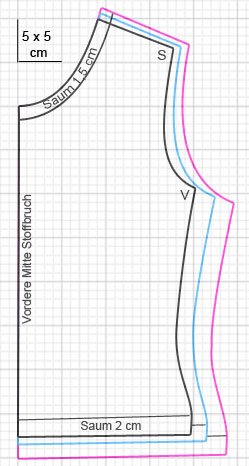
\includegraphics[width=64.54mm]{Front.jpg}
      \caption{Front Pattern}
      \label{fig:Front}
\end{figure}

These are the sample equations for the design
% For single equations
\begin{equation}
 b = h + t\\
\end{equation}

% This is the code for multiple equation
\begin{eqnarray}
%if you want no number to the equation then use \nonumber
a & = & b + c \\
& = & d + e \\
& = & f + g 
\end{eqnarray}
%%%%%%%

%%%%%%%
\subsubsection{Back}

for the back portion all the details are written here

\begin{figure}[ht!]
     \centering
     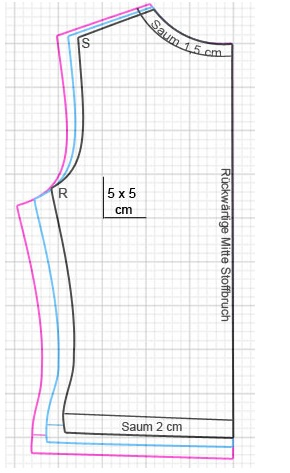
\includegraphics[width=64.54mm]{Back_pattern.jpg}
      \caption{Back Pattern}
      \label{fig:Back}
\end{figure}

These are the equations for back portion
% For single equations
\begin{equation}
 b = h + t\\
\end{equation}


% This is the code for multiple equation
\begin{eqnarray}
%if you want no number to the equation then use \nonumber
a & = & b + c \\
& = & d + e \\
& = & f + g
\end{eqnarray}
%%%%%%%

%%%%%%%
\subsubsection{Sleeve}

for the sleeve portion all the details are written here

\begin{figure}[ht!]
     \centering
     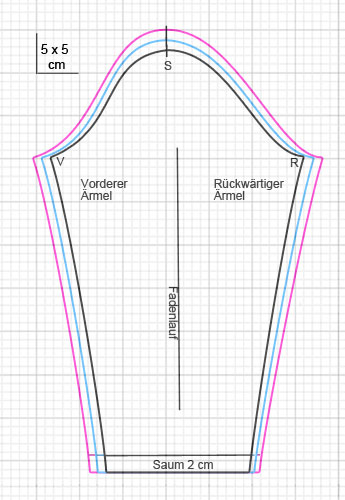
\includegraphics[width=64.54mm]{Sleeve.jpg}
      \caption{Sleeve Pattern}
      \label{fig:Sleeve}
\end{figure}

% For single equations
\begin{equation}
 b = h + t\\
\end{equation}

% This is the code for multiple equation
\begin{eqnarray}
%if you want no number to the equation then use \nonumber
a & = & b + c \\
& = & d + e \\
& = & f + g
\end{eqnarray}
%%%%%%%

%%%%%%
\subsection{Figure Captions}

See figure~\ref{fig:Front} on page~\pageref{fig:Front}.
%%%%%%%

%%%%%%%
\subsection{Table Captions}

See table~\ref{tab:Table 1} for the detailed analysis
%%%%%%%

\end{comment}



\end{document}
